\documentclass[14Q]{jsarticle}
\usepackage[dvipdfmx]{graphicx}
\usepackage{wrapfig}
\usepackage{float}
\usepackage{otf}
\usepackage{longtable}
\usepackage{ulem}
\usepackage{ascmac}
\setlength{\textwidth}{160truemm}      % テキスト幅: 160mm
\setlength{\fullwidth}{\textwidth}     % ページ全体の幅
\setlength{\oddsidemargin}{0mm}   % 左余白
\setlength{\topmargin}{-10mm}       % 上余白
\setlength{\textheight}{240truemm}     % テキスト高さ: 297-(30+30)=237mm
\pagestyle{empty}
\title{北斗市二股台場の調査}% 文書のタイトル
\date{2018年12月3日}
\author{二股台場調査会 野村祐一,塚田直哉,石井淳平}              % 著者
%%%%%%%%%%%%%%%%
\begin{document}
\maketitle
%%%%
\begin{abstract}
北海道の南西部、北斗市の山中の台場山に、「二股台場」(北海道教育委員会の埋蔵文化財包蔵地「台場山遺跡」(B-06-102)として登載)として知られる塹壕の跡が残されており、明治2年(1869)、鶉山道を越えて箱館五稜郭を目指す新政府軍との戦いに備えてここを守備した旧幕府軍が構築したと伝えられている。箱館戦争の戦跡としてだけではなく、城郭史研究の視点からも重要な遺跡である。

本調査ではこれまで知られている台場山の塹壕群の測量を行い、塹壕群の形状と位置の記録を行った。今年度の調査では既知の18箇所の塹壕跡のうち、新発見1箇所を含む6箇所の測量調査を実施し、平面図を作成した。
\end{abstract}

%%%%
\section{二股台場の位置}
北斗市大野町市街地から約10km上流の大野川左岸に位置する。大野川とその支流である二股沢川の合流点付近に位置する。大野市街地から二股沢川付近までは大野川に沿って平坦な地形が続くが、二股台場塹壕群の所在する尾根を境に、これより上流では尾根と谷が交互に現れる急峻な地形となる。

二股台場塹壕群は二股沢川にと並行に北方から大野川にむかって傾斜する尾根上に位置する。最高地点に立地する塹壕(F15)は標高約330m、最低地点に立地する塹壕(F18)は240mである。尾根の鞍部を旧道である「鶉山道」が横切っており、塹壕群は鞍部をはさんで南北に分かれる。

新政府軍の攻撃正面となった尾根の西側斜面は鶉山道南側では平均傾斜約20度、鶉山道北側では約30度である。

\begin{figure}[h]
\centering
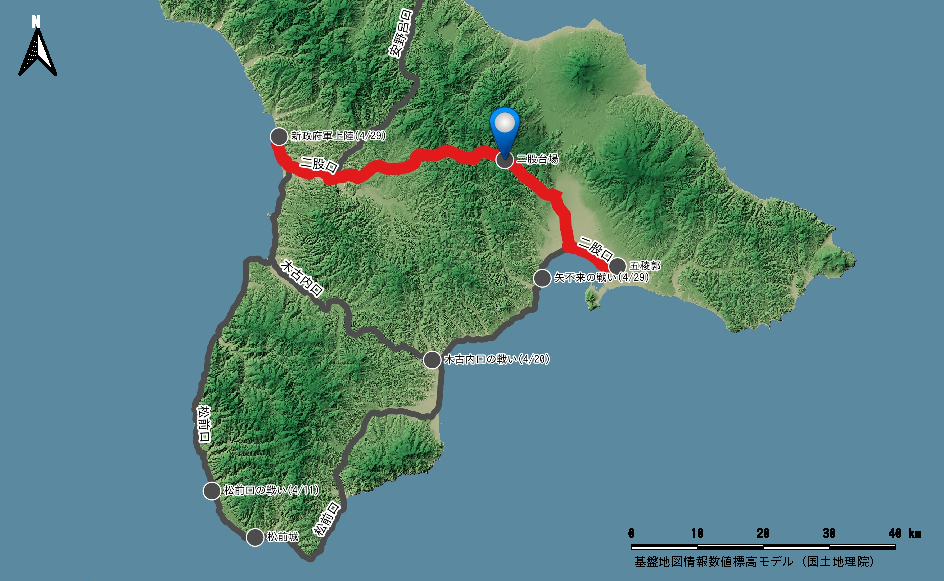
\includegraphics[width=160truemm]{fig/dounan.pdf}
\caption{二股台場の位置と明治2年箱館戦争}
\end{figure}

\begin{figure}[h]
\centering
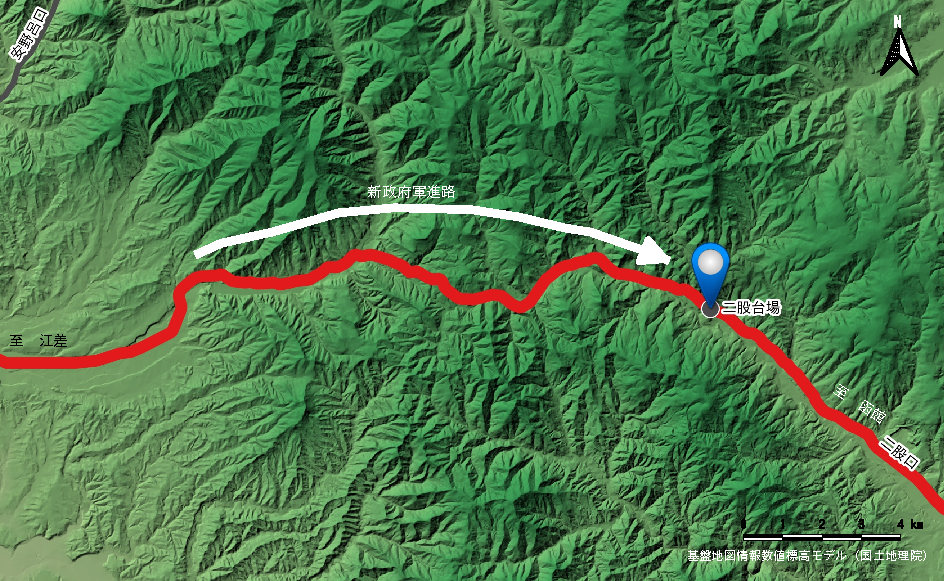
\includegraphics[width=160truemm]{fig/oonoassabu.pdf}
\caption{「鶉山道」と二股台場}
\end{figure}

\begin{figure}[h]
\centering
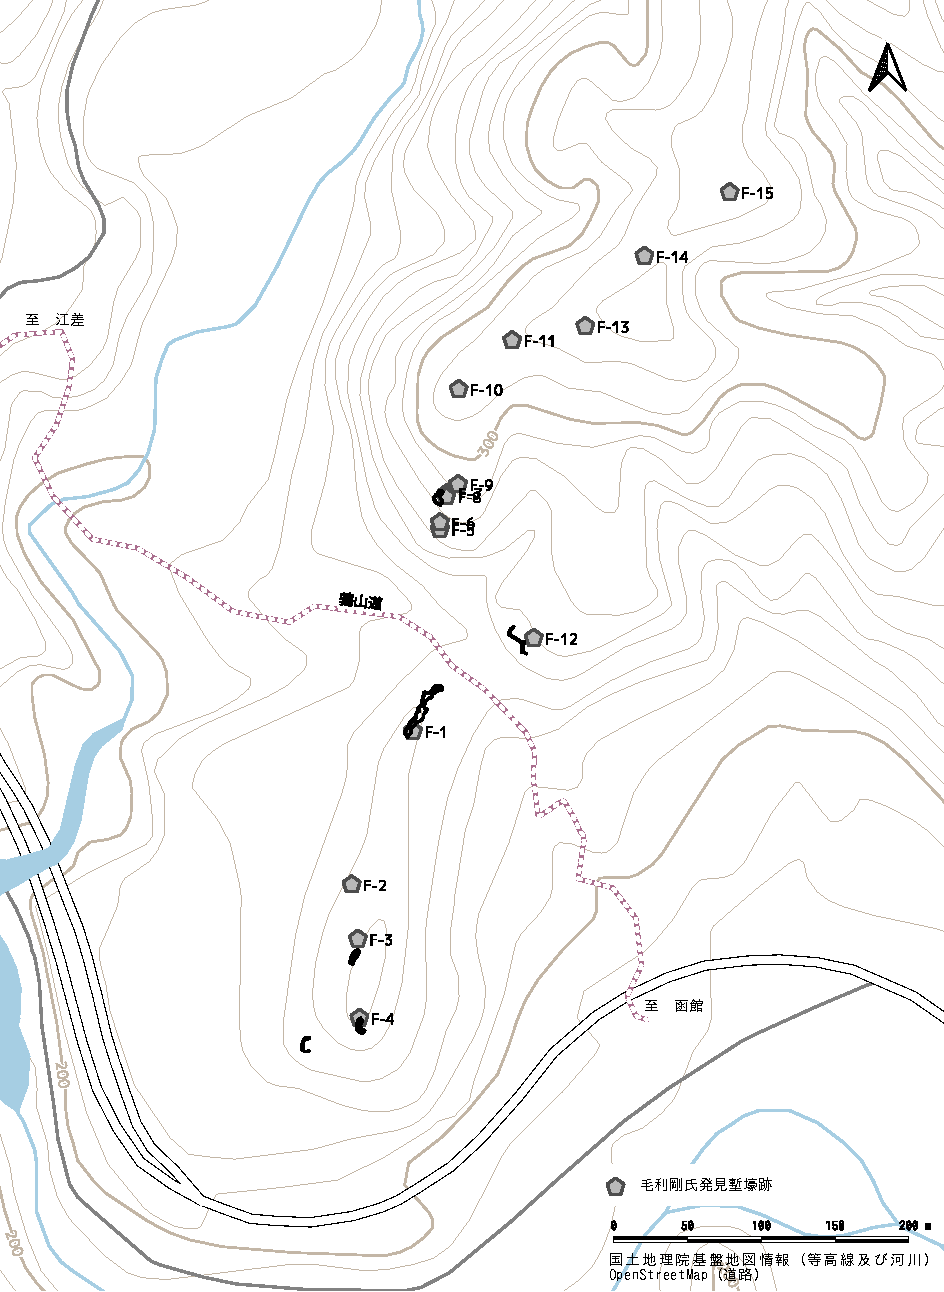
\includegraphics[width=160truemm]{fig/haitizu.pdf}
\caption{二股台場周辺の地形と塹壕配置}
\label{haiti}
\end{figure}

%%%%
\section{箱館戦争と二股台場}
\subsection{明治2年箱館戦争}
明治2年(1869)4月9日に北海道南西部の乙部に上陸した新政府軍は、ただちに西部の要衝である江差を占領した。新政府軍は「松前口」、「二股口」、「木古内口」、「安野呂ロ」の4つの攻撃軸を設定した。このうち、松前城のある「松前口」にもっとも大きな兵力が割かれており、ついで大きな兵力が派遣されたのが、現在の厚沢部町から北斗市を経由して函館市へ至る「二股口」である。

この動きを察知した旧幕府軍は、4月11日頃「台場山」に到着し、ここに陣地を構築する。『北国戦争概略衝鉾隊之記』によると、当初旧幕府軍は大野川左岸の「峠新道」に陣地を構築していたが、新政府軍が旧道を進むとの情報を得たため、台場山に転陣したという。

\subsection{二股口の戦闘}
二股台場に対する新政府軍の攻撃は4月13日の夕方頃とされている(『北国戦争概略衝鉾隊之記』、『南柯紀行』)。夜通しの戦闘の後、新政府軍は退却します。

2度めの戦闘は、4月23日の夕方頃とされる(前掲)。二股台場から3kmほど西側の新政府軍前進陣地付近で旧幕府側の攻撃により戦端が開かれた。退却する旧幕府軍を追って新政府軍の追撃戦が行われ、再び二股台場付近での戦闘となった。戦闘はこの日も夜通し続けられたが、二股台場からの逆襲を受けて新政府軍は敗走する場面もあり、二股台場の攻略に失敗した。

\subsection{二股台場から退却}
その後、二股台場をめぐる大規模な戦闘は行われなかったが、松前口、木古内口での戦況は旧幕府軍にとって次第に悪化した。函館平野の入り口にあたる矢不来の防御戦闘が失敗に終わったことから、二股台場は戦略的な意味を失うこことなった。

4月29日、二股台場を守備していた旧幕府軍は陣地を放棄し、箱館五稜郭へ撤退した。守備隊の撤退により、二股台場は役割を終えることとなる。

%%%%
\section{研究史}
\subsection{河野常吉}

\subsection{毛利剛氏の踏査}

%%%%
\section{調査の方法}
\subsection{基準点の設置}
GPS 磁北
UTM座標系

\subsection{実測の方法}
20分1

\subsection{塹壕名称}
毛利剛氏の踏査


%%%%
\section{調査の経過}


%%%%
\section{塹壕配置}
図\ref{haiti_tate}に示すように、塹壕群は鶉山道で南北に分断される。もっとも長大なF01塹壕は鶉山道の南側で山道に北端を接している。山道北側の塹壕群が山道を見下ろす位置で山道の北側側面に面して配置される。

\begin{figure}[h]
\centering
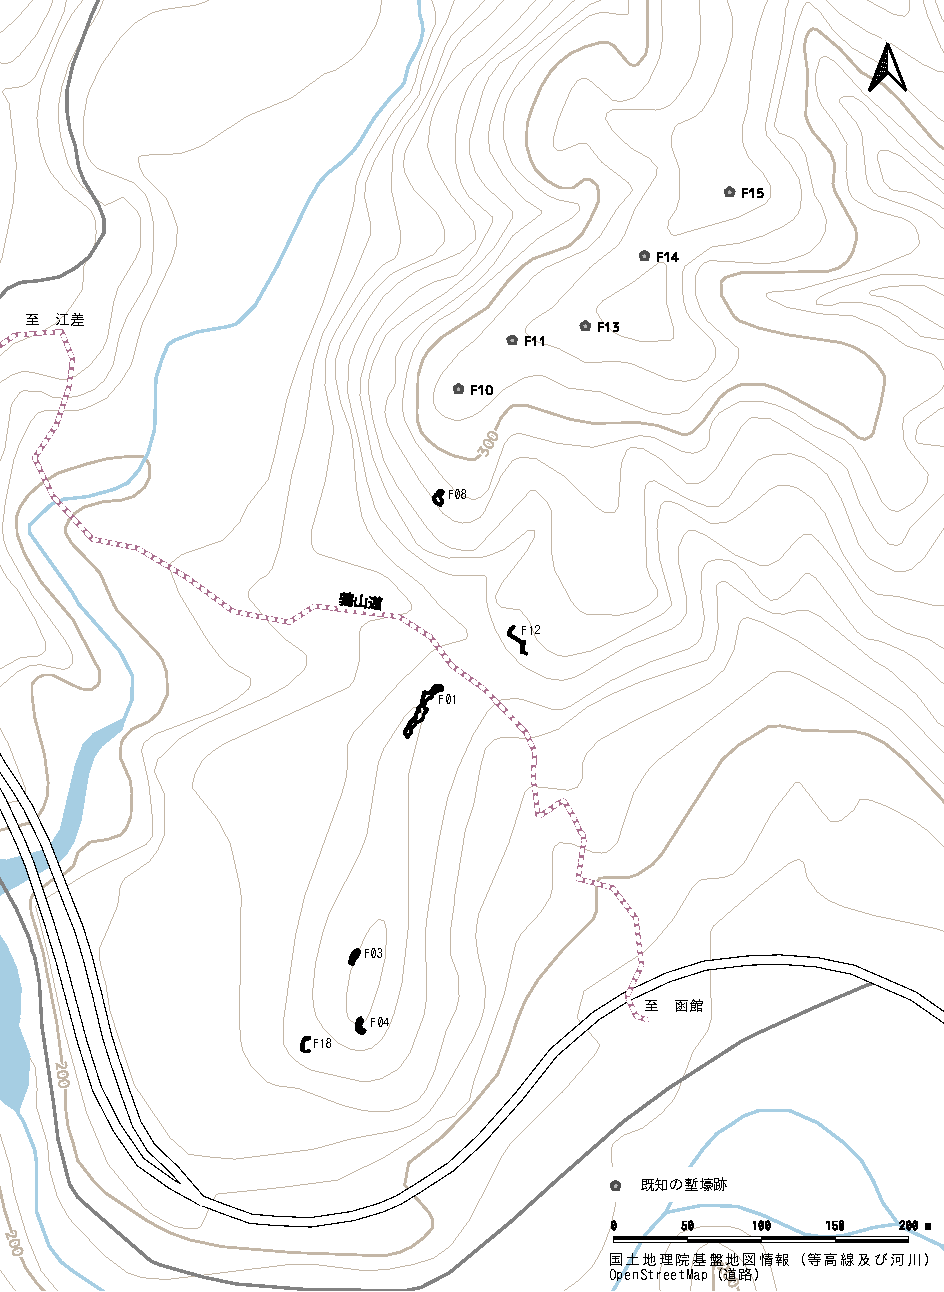
\includegraphics[width=160truemm]{fig/haitizu_tate.pdf}
\caption{塹壕配置}
\label{haiti_tate}
\end{figure}

%%%%
\section{塹壕}
\subsection{F01}
「イナズマ型塹壕」として知られる塹壕である。二股台場塹壕群中もっとも延長が長い。「イナズマ」の由来となった塹壕の屈曲については平面図上では明瞭ではなく、意図的な屈曲というよりも、地形に影響された結果、塹壕が湾曲しているようである。ただしX=4643830ライン付近は意図的な突出部と考えられる。

\begin{figure}[h]
\centering
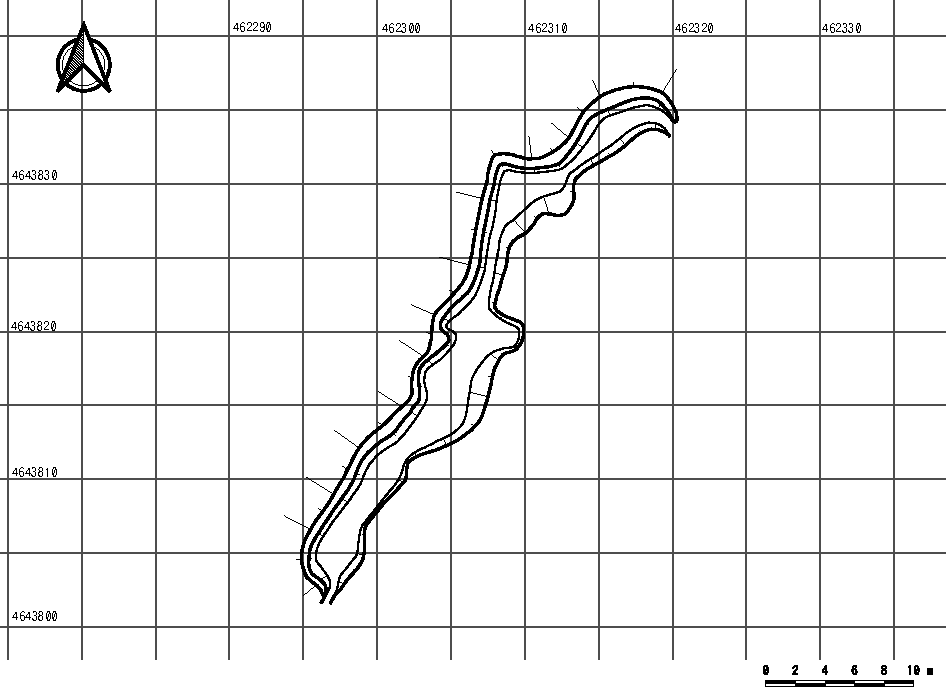
\includegraphics[width=160truemm]{fig/F01.pdf}
\caption{F01塹壕}
\label{f01}
\end{figure}

%%%%
\subsection{F03塹壕}
F01塹壕南西、直線距離で約150m離れる。毛利剛氏の踏査ではF01塹壕とF03塹壕の間にF02塹壕が確認されているが、今回の調査ではハケ検できなかった。

\begin{figure}[h]
\centering
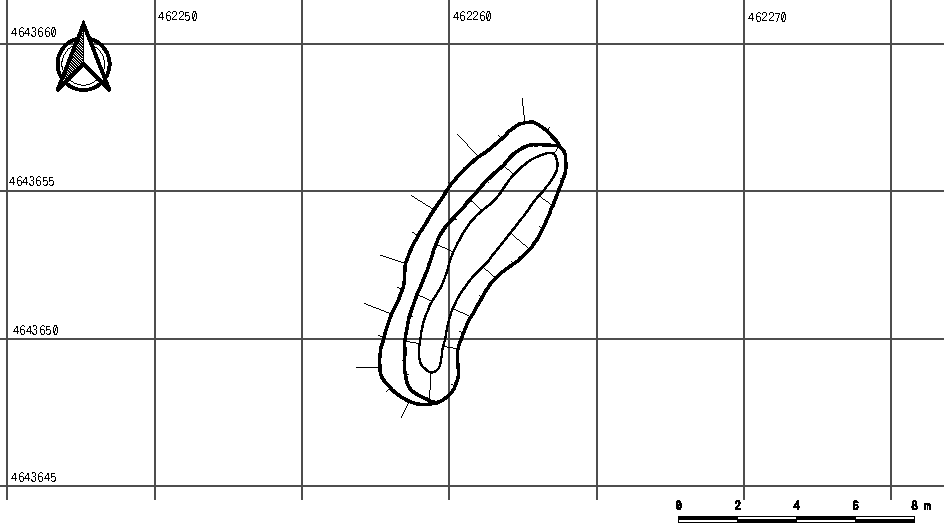
\includegraphics[width=160truemm]{fig/F03.pdf}
\caption{F03塹壕}
\label{f01}
\end{figure}

%%%%
\subsection{F04塹壕}

\begin{figure}[h]
\centering
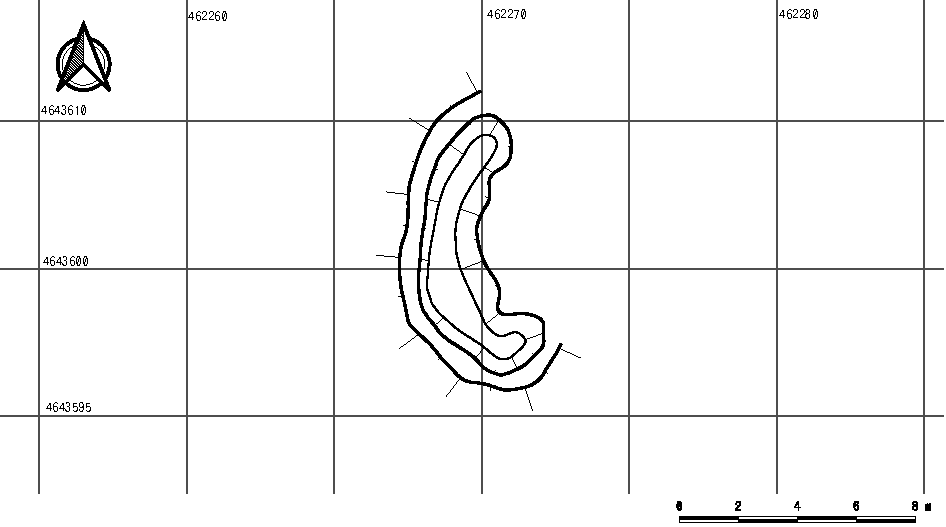
\includegraphics[width=160truemm]{fig/F04.pdf}
\caption{F04塹壕}
\label{f04}
\end{figure}

%%%%
\subsection{F18塹壕}

\begin{figure}[h]
\centering
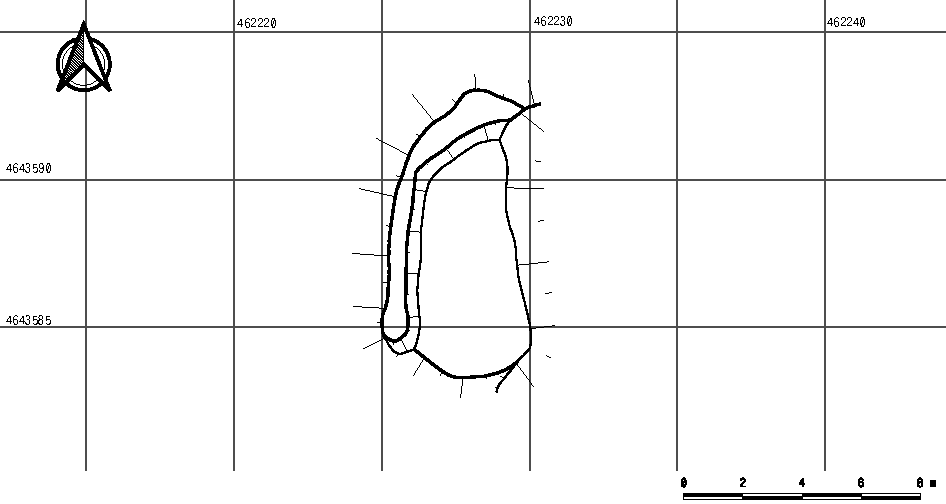
\includegraphics[width=160truemm]{fig/F18.pdf}
\caption{F18塹壕}
\label{f18}
\end{figure}

%%%%
\subsection{F12塹壕}

\begin{figure}[h]
\centering
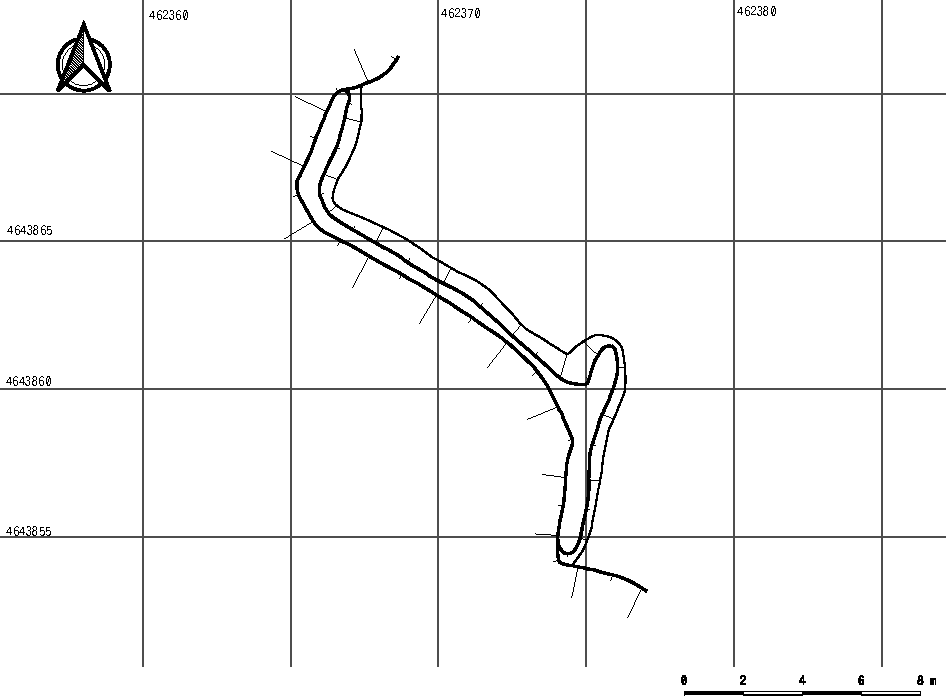
\includegraphics[width=160truemm]{fig/F12.pdf}
\caption{F12塹壕}
\label{f12}
\end{figure}

%%%%
\subsection{F08塹壕}

\begin{figure}[h]
\centering
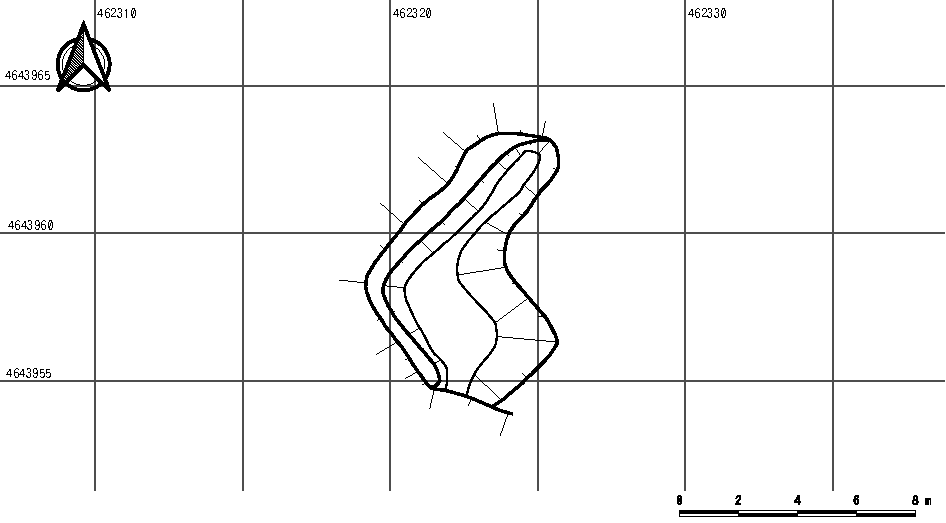
\includegraphics[width=160truemm]{fig/F08.pdf}
\caption{F08塹壕}
\label{f08}
\end{figure}

\end{document}
